\documentclass[10pt,twocolumn,letterpaper]{article}

\usepackage{cvpr}
\usepackage{times}
\usepackage{epsfig}
\usepackage{graphicx}
\usepackage{amsmath}
\usepackage{amssymb}
\usepackage{subfigure}
\usepackage{upgreek}
\usepackage{multirow}
\usepackage{color}
\usepackage{bm}
\DeclareMathOperator*{\argmin}{arg\,min}
\usepackage{arydshln}

% Include other packages here, before hyperref.

% If you comment hyperref and then uncomment it, you should delete
% egpaper.aux before re-running latex.  (Or just hit 'q' on the first latex
% run, let it finish, and you should be clear).
\usepackage[pagebackref=true,breaklinks=true,letterpaper=true,colorlinks,bookmarks=false]{hyperref}

% \cvprfinalcopy % *** Uncomment this line for the final submission

\def\cvprPaperID{****} % *** Enter the CVPR Paper ID here
\def\httilde{\mbox{\tt\raisebox{-.5ex}{\symbol{126}}}}

% Pages are numbered in submission mode, and unnumbered in camera-ready
\ifcvprfinal\pagestyle{empty}\fi


\begin{document}

%%%%%%%%% TITLE
\title{External Patch Group Prior Guided Internal Prior Learning for Real Image Denoising}

\author{First Author\\
Institution1\\
Institution1 address\\
{\tt\small firstauthor@i1.org}
% For a paper whose authors are all at the same institution,
% omit the following lines up until the closing ``}''.
% Additional authors and addresses can be added with ``\and'',
% just like the second author.
% To save space, use either the email address or home page, not both
\and
Second Author\\
Institution2\\
First line of institution2 address\\
{\tt\small secondauthor@i2.org}
}

\maketitle 


%%%%%%%%% ABSTRACT
\begin{abstract}
For image denoising problem, the external and internal priors are playing key roles in many different methods. External priors learn from external images to restore noisy images while internal ones exploit priors of given images for denoising. The external priors are more generative and efficient on recovering structure s existing in most images while the internal priors are more adaptive on recovering details existed in given noisy images. In this paper, we propose to employ the external patch group prior of images to guide the clustering of internal patch groups, and develop an external dictionary guided internal orthogonal dictionary learning algorithm for real image denoising. The internal orthogonal dictionary learning process has closed-form solutions and hence very efficient for image denoising. We perform extensive experiments on dozens of real noisy images captured by different cameras and camera settings under controlled indoor or uncontrolled outdoor lighting conditions. The results demonstrate that the proposed method achieves better performance than other state-of-the-art methods on real image denoising. 
\end{abstract}
%Though these methods are very effective in Gaussian noise removal, the noise in real images are signal dependent and more complex than Gaussian noise. Therefore, only exploiting the external or internal priors are not enough for real image denoising.

%%%%%%%%% BODY TEXT
\section{Introduction} 

Most vision systems, such as medical imaging and surveillance, need accurate feature extraction from high-quality images. The camera sensors and outdoor low light conditions will unavoidably bring noise to the captured images. The impact is that the image details will be lost or hardly visible. As a result, image denoising is an essential procedure for the reliability of these vision systems. In the research area, image denoising is also an ideal platform for testing natural image models and provides high-quality images for other computer vision tasks such as image registration, segmentation, and pattern recognition. 

For several decades, there emerge numerous image denoising methods \cite{nlm,foe,ksvd,bm3d,cbm3d,lssc,epll,mlp,wnnm,csf,pgpd,chen2015learning}, and all of them focus mainly on dealing with additive white Gaussian noise (AWGN). In real world, the cameras will undertake high ISO settings for high-speed shots on actions, long exposure for low light on night shots, etc. Under these situations, the noise is generated in a complex form and also been changed during the in-camera imaging pipeline \cite{NewInCamera,crosschannel2016}. Therefore, the noise in real images are much more complex than Gaussian \cite{crosschannel2016,healey1994radiometric}. It depends on camera series, brands, as well as the settings (ISO, shutter speed, and aperture, etc.). The models designed for AWGN would become much less effective on real noisy images. 

In the last decade, the methods of \cite{fullyblind,rabie2005robust,Liu2008,almapg,noiseclinic,ncwebsite,Zhu_2016_CVPR,crosschannel2016} are developed to deal with real noisy images. Almost all these methods employ a two-stage framework: estimating the parameters of the assumed noise model (usually Gaussian) and performing denoising with the help of the noise modeling and estimation in the first stage. However, the Gaussian assumption is inflexible in describing the complex noise on real noisy images \cite{Liu2008}. Although the mixture of Gaussians (MoG) model is possible to approximate any noise distribution \cite{Bishop}, estimating its parameters is time consuming via nonparametric Bayesian techniques \cite{Zhu_2016_CVPR}. To evaluate the performance of these methods on dealing with complex real noise, we apply these methods, with corresponding default parameters, on a real noisy image provided in \cite{crosschannel2016}. The testing image is captured by a Nikon D800 camera when ISO is 3200. The "ground truth" image is also provided with which we can calculate objective measurements such as PSNR. The denoised images are listed in Figure \ref{fig1}, from which we can see that these methods either remove the noise or over-smooth the complex details in real noisy image. 
\begin{figure*}
\centering
\subfigure{
\begin{minipage}[t]{0.195\textwidth}
\centering
\raisebox{-0.15cm}{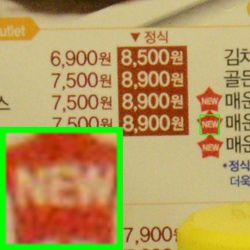
\includegraphics[width=1\textwidth]{images/resize_br_Noisy_CC_Noisy_Nikon_D800_ISO_3200_A3_66.png}}
{\footnotesize (a) Noisy \cite{crosschannel2016}: 33.30dB }
\end{minipage}
\begin{minipage}[t]{0.195\textwidth}
\centering
\raisebox{-0.15cm}{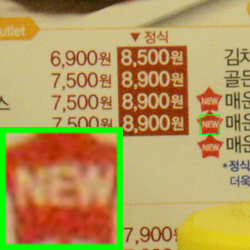
\includegraphics[width=1\textwidth]{images/resize_br_CBM3D_CC_Noisy_Nikon_D800_ISO_3200_A3_66.png}}
{\footnotesize (b) BM3D \cite{bm3d,cbm3d}: 33.33dB  }
\end{minipage}
\begin{minipage}[t]{0.195\textwidth}
\centering
\raisebox{-0.15cm}{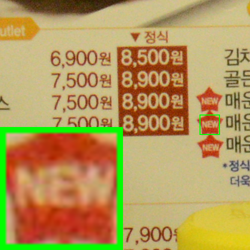
\includegraphics[width=1\textwidth]{images/resize_br_WNNM_CC_Noisy_Nikon_D800_ISO_3200_A3_66.png}}
{\footnotesize (c) WNNM \cite{wnnm}: 33.30dB  }
\end{minipage}
\begin{minipage}[t]{0.195\textwidth}
\centering
\raisebox{-0.15cm}{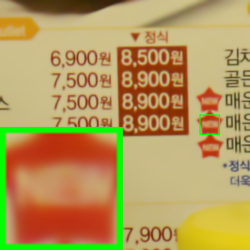
\includegraphics[width=1\textwidth]{images/resize_br_MLP_CC_Noisy_Nikon_D800_ISO_3200_A3_66.png}}
{\footnotesize (d) MLP \cite{mlp}: 34.22dB }
\end{minipage}
\begin{minipage}[t]{0.195\textwidth}
\centering
\raisebox{-0.15cm}{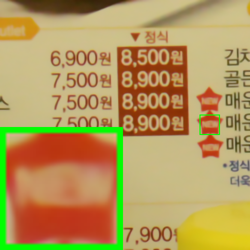
\includegraphics[width=1\textwidth]{images/resize_br_CSF_CC_Noisy_Nikon_D800_ISO_3200_A3_66.png}}
{\footnotesize (e) CSF \cite{csf}: 35.39dB }
\end{minipage}
}\vspace{-3mm}
\subfigure{
\begin{minipage}[t]{0.195\textwidth}
\centering
\raisebox{-0.15cm}{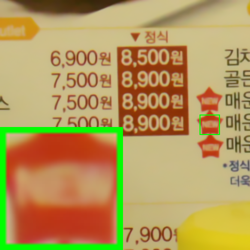
\includegraphics[width=1\textwidth]{images/resize_br_TRD_CC_Noisy_Nikon_D800_ISO_3200_A3_66.png}}
{\footnotesize (f) TRD \cite{chen2015learning}: 35.97dB   }
\end{minipage}
\begin{minipage}[t]{0.195\textwidth}
\centering
\raisebox{-0.15cm}{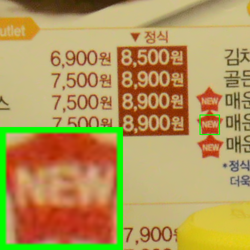
\includegraphics[width=1\textwidth]{images/resize_br_NC_CC_Noisy_Nikon_D800_ISO_3200_A3_66.png}}
{\footnotesize (g) NC \cite{noiseclinic}: 35.33dB  }
\end{minipage}
\begin{minipage}[t]{0.195\textwidth}
\centering
\raisebox{-0.15cm}{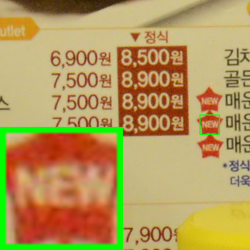
\includegraphics[width=1\textwidth]{images/resize_br_NI_CC_Noisy_Nikon_D800_ISO_3200_A3_66.png}}
{\footnotesize (h) NI \cite{neatimage}: 34.39dB  }
\end{minipage}
\begin{minipage}[t]{0.195\textwidth}
\centering
\raisebox{-0.15cm}{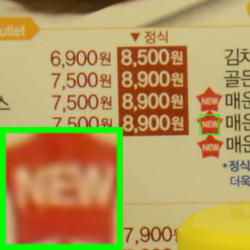
\includegraphics[width=1\textwidth]{images/resize_br_Guided_CC_Noisy_Nikon_D800_ISO_3200_A3_66.png}}
{\footnotesize (i) Ours: \textbf{37.02}dB  }
\end{minipage}
\begin{minipage}[t]{0.195\textwidth}
\centering
\raisebox{-0.15cm}{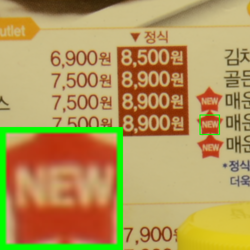
\includegraphics[width=1\textwidth]{images/resize_br_Mean_CC_Noisy_Nikon_D800_ISO_3200_A3_66.png}}
{\footnotesize (j) Mean Image \cite{crosschannel2016} }
\end{minipage}
}\vspace{-1mm}
\caption{Denoised images of the real noisy image "Nikon D800 ISO 3200 A3" from \cite{crosschannel2016} by different methods. The images are better viewed by zooming in on screen.} 
\vspace{-3mm}
\label{fig1}
\end{figure*}

The above mentioned methods can be categorized into external methods which learn priors from external images to recover noisy images, and internal ones which exploit priors of given images for denoising. The external priors in natural images are free of the high correlation between noise and signals in real noisy images, while the internal prior is adaptive to the image and can recover better the latent clean image. Combining the priors of external clean images and priors of internal testing images can naturally improve the performance of denoising methods, especially on real noisy images. Based on these observations, in this paper, we propose to employ the external patch group prior \cite{pgpd} of natural clean images to guide the clustering of internal patch groups in given noisy image, and develop an external prior guided internal orthogonal dictionary learning (DL) algorithm for real image denoising. The internal orthogonal DL process includes two alternating stages: updating sparse coefficients and updating orthogonal dictionary. Both of the two stages have closed-form solutions. Hence, our internal DL process is very efficient for online internal denoising. Through comprehensive experiments on real noisy images captured by different cameras and settings, we demonstrate that the proposed method achieves better performance on real image denoising

\subsection{Our Contributions}

The contributions of this paper are summarized as follows:
\begin{itemize}
\item We propose a novel model to learn internal priors adaptive to given images. This model employs the external patch group (PG) prior learned from clean images to guide the internal PG prior learning of given images. The external prior benefits the internal learning on subspace selection and orthogonal dictionary learning.
\item The proposed guided internal prior learning method is very efficient. The reason is that both the subspace selection and orthogonal dictionary learning have explicit solutions.
\item For real image denoising problem, the proposed method achieves much better performance than other competing methods.
\end{itemize}

The rest of this paper will be summarized as follows: in Section 2, we briefly introduce the related work; in Section 3, we develop the proposed external prior guided internal prior learning model and formulate the overall image denoising algorithm; in Section 3, we demonstrate extensive experiments on real image denoising problem; in Section 4, we conclude our paper and give future work.

\section{Related Work}

\begin{figure*}
\centering
\subfigure{
\begin{minipage}[t]{0.195\textwidth}
\centering
\raisebox{-0.15cm}{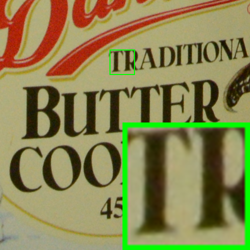
\includegraphics[width=1\textwidth]{images/resize_br_Noisy_CC_Noisy_Nikon_D600_ISO_3200_C1_96.png}}
{\footnotesize (a) Noisy \cite{crosschannel2016}: 35.89dB  }
\end{minipage}
\begin{minipage}[t]{0.195\textwidth}
\centering
\raisebox{-0.15cm}{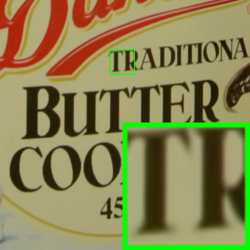
\includegraphics[width=1\textwidth]{images/resize_br_Offline_CC_Noisy_Nikon_D600_ISO_3200_C1_96.png}}
{\footnotesize (b) External: 39.05dB }
\end{minipage}
\begin{minipage}[t]{0.195\textwidth}
\centering
\raisebox{-0.15cm}{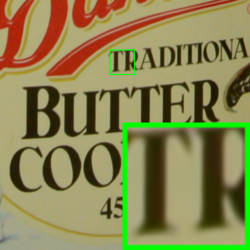
\includegraphics[width=1\textwidth]{images/resize_br_Online_CC_Noisy_Nikon_D600_ISO_3200_C1_96.png}}
{\footnotesize (c) Internal: 38.75dB }
\end{minipage}
\begin{minipage}[t]{0.195\textwidth}
\centering
\raisebox{-0.15cm}{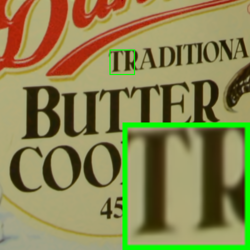
\includegraphics[width=1\textwidth]{images/resize_br_Guided_CC_Noisy_Nikon_D600_ISO_3200_C1_96.png}}
{\footnotesize (d) Ours: \textbf{39.39}dB }
\end{minipage}
\begin{minipage}[t]{0.195\textwidth}
\centering
\raisebox{-0.15cm}{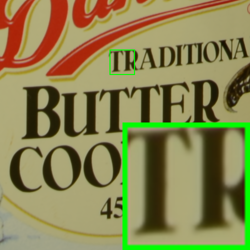
\includegraphics[width=1\textwidth]{images/resize_br_Mean_CC_Noisy_Nikon_D600_ISO_3200_C1_96.png}}
{\footnotesize (e) Mean Image \cite{crosschannel2016}}
\end{minipage}
}
\caption{Denoised images of the $96$-th cropped image from "Nikon D600 ISO 3200 C1" \cite{crosschannel2016} by different methods. The images are better to be zoomed in on screen.}
\vspace{-3mm}
\label{fig2}
\end{figure*}

\subsection{Patch Group Prior of Natural Images}

The Patch Group (PG) prior \cite{pgpd} is proposed to directly model the non-local self-similarity (NSS) property of natural images. The NSS property is commonly used in image restoration tasks \cite{nlm,bm3d,lssc,wnnm,pgpd}. The PG prior largely reduces the space of images to be modeled when compared to the patch prior \cite{epll}. In \cite{pgpd}, only the PGs of clean natural images is utilized, while the PGs of noisy input images are ignored. In this paper, we make use of PGs both from external clean images and internal given real noisy image for better denoising performance.

\subsection{Internal v.s. External Prior Learning}

Learning priors to represent images has been successfully used in image modeling \cite{ksvd,epll,pgpd,ple,ncsr}. There are mainly two categories of prior learning methods: 1) External methods pre-learned priors (e.g., dictionaries) from a set of clean images, and the learned priors are used to recover the noisy images \cite{epll,pgpd}. 2) Internal methods directly learned priors from the given noisy image, and the image denoising is simultaneously done with the learning process \cite{ksvd,ple,ncsr}. Both the two categories of methods have limitations. The external methods is not adaptive to the noisy image, while the internal methods ignores the information hidden in clean images. In this paper, our goal is to employ the external prior to guide the internal prior learning.

\subsection{Real Image Denoising}

In the last decade, researchers proposed many methods \cite{fullyblind,rabie2005robust,Liu2008,almapg,noiseclinic,ncwebsite,Zhu_2016_CVPR,crosschannel2016} for real image denoising problem. In \cite{fullyblind}, Portilla proposed to use scale mixture of Gaussian to estimate the noise covariance matrix and latent clean images in wavelet domain. The work of Rabie \cite{rabie2005robust} modeled the noisy pixels as outliers which are removed via Lorentzian robust estimator \cite{huber2011robust}. Liu et al. \cite{Liu2008} proposed to use 'noise level function' to estimate the noise and then use Gaussian conditional random field to obtain the latent clean image. Gong et al. \cite{almapg} models the noise by mixed $\ell_{1}$ and $\ell_{2}$ norms and remove the noise by sparsity prior in the wavelet transform domain. Later, Lebrun el al. proposed a multiscale denoising algorithm called 'Noise Clinic' \cite{noiseclinic,ncwebsite}. This method generalizes the NL-Bayes model \cite{nlbayes} to deal with blind noise and achieves state-of-the-art performance. Recently, Zhu et al. proposed a Bayesian model \cite{Zhu_2016_CVPR} which approximates and removes the noise via Low-Rank Mixture of Gaussians.

\section{External Patch Group Prior Guided Internal Prior Learning for Image Denoising}

\begin{figure*}
\centering
\subfigure{
\begin{minipage}[t]{0.195\textwidth}
\centering
\raisebox{-0.15cm}{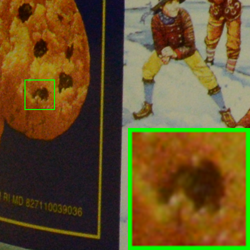
\includegraphics[width=1\textwidth]{images/resize_br_Noisy_CC_Noisy_Nikon_D600_ISO_3200_C1_94.png}}
{\footnotesize (a) Noisy \cite{crosschannel2016}: 34.55dB  }
\end{minipage}
\begin{minipage}[t]{0.195\textwidth}
\centering
\raisebox{-0.15cm}{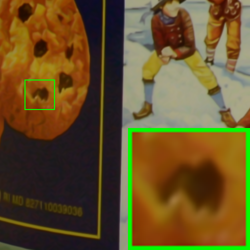
\includegraphics[width=1\textwidth]{images/resize_br_Offline_CC_Noisy_Nikon_D600_ISO_3200_C1_94.png}}
{\footnotesize (b) External: 36.09dB }
\end{minipage}
\begin{minipage}[t]{0.195\textwidth}
\centering
\raisebox{-0.15cm}{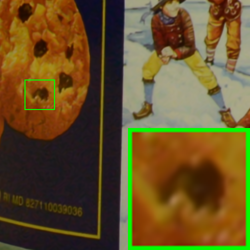
\includegraphics[width=1\textwidth]{images/resize_br_Online_CC_Noisy_Nikon_D600_ISO_3200_C1_94.png}}
{\footnotesize (c) Internal: 37.11dB }
\end{minipage}
\begin{minipage}[t]{0.195\textwidth}
\centering
\raisebox{-0.15cm}{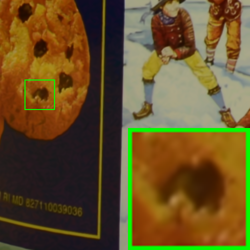
\includegraphics[width=1\textwidth]{images/resize_br_Guided_CC_Noisy_Nikon_D600_ISO_3200_C1_94.png}}
{\footnotesize (d) Ours: \textbf{37.39}dB }
\end{minipage}
\begin{minipage}[t]{0.195\textwidth}
\centering
\raisebox{-0.15cm}{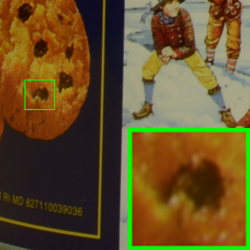
\includegraphics[width=1\textwidth]{images/resize_br_Mean_CC_Noisy_Nikon_D600_ISO_3200_C1_94.png}}
{\footnotesize (e) Mean Image \cite{crosschannel2016}}
\end{minipage}
}
\caption{Denoised images of the $94$-th cropped image from "Nikon D600 ISO 3200 C1" \cite{crosschannel2016} by different methods. The images are better to be zoomed in on screen.}
\vspace{-3mm}
\label{fig3}
\end{figure*}


In this section, we formulate the framework of external patch group (PG) prior guided internal prior learning. We first introduce the external PG prior leaning on natural clean RGB images. Then we propose to employ the learned external PG prior to guide the internal prior (subspace selection and dictionary learning (DL)) learning of given degraded (such as noisy) images. Under the weighted sparse coding framework, the internal prior learning process has alternative closed-form solutions in term of updating sparse coefficients and orthogonal dictionary. Finally, we discuss in details how external prior learned from natural clean images guide the internal prior learning of given degraded (noisy) images.

\subsection{External Patch Group Prior Learning}

Natural images often demonstrate repetitive local patterns, this nonlocal self-similarity (NSS) property is a key successful factor for many image denoising methods \cite{nlm,bm3d,lssc,ncsr,wnnm,pgpd}. In this section, we formulate the Patch Group prior learned on natural color images. Similar to \cite{pgpd}, the patch group (PG) is defined as a group of similar patches to the local patch. The patch group mean is subtracted, and hence different groups patches can share similar PGs. In this way, the space natural image patches to be modeled is largely reduced. 

In this work, each local patch extracted from RGB images is of size $p\times p \times 3$. Then we search the $M$ most similar patches $\{\mathbf{x}_{m}\}_{m=1}^{M}$ around each local patch through Euclidean distance, in a local window of size $W\times W$. The $\mathbf{x}_{m}\in \mathbb{R}^{3p^{2}\times1}$ is a patch vector formed by combining the 3 patch vectors (of size $p^{2}\times 1$) in R, G, B channels. The mean vector of this PG is $\boldsymbol{\upmu}=\frac{1}{M}\sum_{m=1}^{M}\mathbf{x}_{m}$, and the group mean subtracted PG is defined as $\mathbf{\overline{X}}\triangleq \{\mathbf{\overline{x}}_{m}=\mathbf{x}_{m}-\boldsymbol{\upmu}\}, m=1,...,M$. Assume we have extracted $N$ PGs from a set of external natural images, and the $n$-th PG is defined as $\mathbf{\overline{X}}_{n}\triangleq \{\mathbf{\overline{x}}_{n,m}\}_{m=1}^{M}, n=1,...,N$. We employ the Gaussian Mixture Model (GMM) to learn the external patch group based NSS prior. In this model, the likelihood of the $n$-th PG $\{\mathbf{\overline{X}}_{n}\}$ can be calculated as
\vspace{-2mm}
\begin{equation}\label{equ1}\vspace{-2mm}
P(\mathbf{\overline{X}}_{n})  = \sum\nolimits_{k=1}^{K}\pi_{k}\prod\nolimits_{m=1}^{M}\mathcal{N}(\mathbf{\overline{x}}_{n,m}|\boldsymbol{\upmu}_{k},\mathbf{\Sigma}_{k}),
\end{equation}
where $K$ is the number of Gaussians and the parameters $\pi_{k}$, $\boldsymbol{\upmu}_{k}$, $\mathbf{\Sigma}_{k}$ are mixture weight, mean vector, and covariance matrix of the $k$-th Gaussian, respectively. By assuming that all the PGs are independently sampled, the overall objective log-likelihood function is
\vspace{-2mm}
\begin{equation}\label{equ2}\vspace{-2mm}
\begin{split}
\ln\mathcal{L}=\sum_{n=1}^{N} \ln(\sum_{k=1}^{K}\pi_{k}\prod_{m=1}^{M}\mathcal{N}(\mathbf{\overline{x}}_{n,m}|\boldsymbol{\upmu}_{k},\mathbf{\Sigma}_{k})).
\end{split}
\end{equation} 
We maximize the above objective function via EM algorithm \cite{em} and finally obtain the GMM model with learned parameters. Similar to \cite{pgpd}, the mean vector of each cluster is natural zeros, i.e., $\boldsymbol{\upmu}_{k}=\mathbf{0}$.

Now, we have clustered the PGs extracted from external clean images into $K$ Gaussians or subspaces. To better characterize each subspace, we perform singular value decomposition (SVD) on the covariance matrix:
\vspace{-2mm}
\begin{equation}\label{equ3}\vspace{-2mm}
\mathbf{\Sigma}_{k}=\mathbf{U}_{k}\mathbf{S}_{k}\mathbf{U}_{k}^{\top}.
\end{equation}
The singular vector matrices $\{\mathbf{U}_{k}\}_{k=1}^{K}$ are employed as the external orthogonal dictionary to guide the internal dictionary learning. The singular values in the diagonal of $\mathbf{S}_{k}$ reflect the significance of the singular vectors in $\mathbf{U}_{k}$ and utilized as prior weights for weighted sparse coding which will be discussed in next section.

\subsection{External Prior Guided Internal Prior Learning}

After the external patch group (PG) prior is learned, we can employ it to guide the internal PG prior learning for the given testing (real noisy) image. The guidance mainly comes from two aspects. One aspect is that the external prior can guide the internal noisy PGs to be assigned to most suitable Gaussians or subspaces. And for each subspace, the other aspect is to guide the orthogonal dictionary learning of internal noisy PGs.

\vspace{-2mm}
\subsubsection{Guided Internal Subspace Selection}
\vspace{-1mm}

Given a real noisy image, assume we can totally extract $N$ local patches from it. Similar to the external prior learning stage, for the $n$-th local patch ($n=1,...,N$), we extract its $M$ most similar patches around it to form a noisy PG denoted by $\mathbf{Y}_{n} = \{\mathbf{y}_{n,1},...,\mathbf{y}_{n,M}\}$. Then the group mean of $\mathbf{Y}_{n}$, denoted by $\bm{\mu}_{n}$, is calculated and subtracted from each patch by $\mathbf{\overline{y}}_{n,m}=\mathbf{y}_{n,m}-\bm{\mu}_{n}$, leading to the mean subtracted PG $\mathbf{\overline{Y}}_{n}\triangleq \{\mathbf{\overline{y}}_{n,m}\}_{m=1}^{M}$. For adaptivity, we project the PG $\mathbf{\overline{Y}}_{n}$ into its most suitable Gaussian component (subspace) of the GMM learned on external PGs. The subspace most suitable for $\mathbf{\overline{Y}}_{n}$ is selected by firstly calculating the posterior probability of "$\mathbf{\overline{Y}}_{n}$ belonging to the $k$th Gaussian component":
\vspace{-2mm}
\begin{equation}\label{equ4}\vspace{-1mm}
P(k|\mathbf{\overline{Y}}_{n})=\frac{\prod_{m=1}^{M}\mathcal{N}(\mathbf{\overline{y}}_{n,m}|\mathbf{0},\mathbf{\Sigma}_{k})}{\sum_{l=1}^{K}\prod_{m=1}^{M}\mathcal{N}(\mathbf{\overline{y}}_{n,m}|\mathbf{0},\mathbf{\Sigma}_{l})}
\end{equation}
for $k=1,...,K$, and then choosing the component with the maximum A-posteriori (MAP) probability $\max_{k}P(k|\mathbf{\overline{Y}}_{n})$.

\vspace{-2mm}
\subsubsection{Guided Internal Orthogonal Dictionary Learning}
\vspace{-2mm}

Assume we have assigned all internal noisy PGs $\{\mathbf{\overline{Y}}_{n}\}_{n=1}^{N}$ to their corresponding most suitable Gaussians or subspaces in $\{\mathcal{N}(\mathbf{0},\mathbf{\Sigma}_{k})\}_{k=1}^{K}$. For the $k$-th subspace, assume the noisy PGs assigned to it are $\{\mathbf{\overline{Y}}_{k_{n}}\}_{n=1}^{N_{k}}$ such that $\mathbf{\overline{Y}}_{k_{n}}=[\mathbf{\overline{y}}_{k_{n},1},...,\mathbf{\overline{y}}_{k_{n},M}]$ and $\sum_{k=1}^{K}N_{k}=N$. We utilize the external orthogonal dictionary $\mathbf{U}_{k}$ (Equ. (\ref{equ3})) to guide the learning of an orthogonal dictionary for adaptively characterizing the internal PGs in the $k$-th subspace. The learned dictionary defined as $\mathbf{D}_{k}\triangleq[\mathbf{D}_{k,e}\ \mathbf{D}_{k,i}]\in \mathbb{R}^{3p^2\times 3p^2}$ has two parts: the external part $\mathbf{D}_{k,e}=\mathbf{U}_{k}(:,1:3p^2-r)\in\mathbb{R}^{3p^2\times (3p^2-r)}$ is directly obtained from the external dictionary $\mathbf{U}_{k}$, and the internal part $\mathbf{D}_{k,i}$ is consisted of dictionary atoms adaptively learned from the internal noisy PGs $\{\mathbf{\overline{Y}}_{k_{n}}\}_{n=1}^{N_{k}}$. For notation simplicity, we ignore the subspace index $k$ and denote the noisy PGs assigned to each subspace as $\mathbf{Y}\triangleq\{\mathbf{\overline{Y}}_{n}\}_{n=1}^{N} = [\mathbf{\overline{y}}_{1,1},...,\mathbf{\overline{y}}_{1,M},...,\mathbf{\overline{y}}_{N,1},...,\mathbf{\overline{y}}_{N,M}]$. The learning is performed under the weighted sparse coding framework proposed as follows:
\vspace{-2mm}
\begin{equation}\label{equ5}\vspace{-3mm}
\begin{split}
&\min_{\mathbf{D}_{i},\{\bm{\alpha}_{n,m}\}}
\sum_{n=1}^{N}\sum_{m=1}^{M}(\|\mathbf{\overline{y}}_{n,m}-\mathbf{D}\bm{\alpha}_{n,m}\|_{2}^{2}+\sum_{j=1}^{3p^{2}}\lambda_{j}|\bm{\alpha}_{n,m,j}|)
\\
&
\text{s.t.}
\quad
\mathbf{D}=[\mathbf{D}_{e}\ \mathbf{D}_{i}],\ \mathbf{D}_{i}^{\top}\mathbf{D}_{i} = \mathbf{I}_{r},\ \mathbf{D}_{e}^{\top}\mathbf{D}_{i} = \mathbf{0},
\end{split}
\end{equation}
where $\bm{\alpha}_{n,m}$ is the sparse coefficient vector of the $m$-th patch $\mathbf{\overline{y}}_{n,m}$ in the $n$-th PG $\mathbf{\overline{Y}}_{n}$ and $\bm{\alpha}_{n,m,j}$ is the $j$-th element of $\bm{\alpha}_{n,m}$. $\lambda_{j}$ is the $j$-th regularization parameter defined as
\vspace{-1mm}
\begin{equation}\label{equ6}\vspace{-1mm}
\lambda_{j} = \lambda/(\sqrt{\mathbf{S}_{j}}+\varepsilon).
\end{equation}
We employ square roots of the singular values in $\mathbf{S}$ (please refer to Equ. (\ref{equ3})) as external prior weights and add a small positive number $\varepsilon$ to avoid zero denominator. Noted that $\mathbf{D}_{e}=\emptyset$ if $r=3p^{2}$ and $\mathbf{D}_{e}=\mathbf{U}_{k}$ if $r=0$. The dictionary $\mathbf{D} = [\mathbf{D}_{e}\ \mathbf{D}_{i}]$ is orthogonal by checking that:
\vspace{-2mm}
\begin{equation}\label{equ7}\vspace{-1mm}
\mathbf{D}^{\top}\mathbf{D} = 
\left[\begin{array}{c}
\mathbf{D}_{e}^{\top}
\\
\mathbf{D}_{i}^{\top}
\end{array}\right]
[\mathbf{D}_{e}\ \mathbf{D}_{i}]
=
\left[\begin{array}{cc}
\mathbf{D}_{e}^{\top}\mathbf{D}_{e}\ \mathbf{D}_{e}^{\top}\mathbf{D}_{i}
\\
\mathbf{D}_{i}^{\top}\mathbf{D}_{e}\ \mathbf{D}_{i}^{\top}\mathbf{D}_{i}
\end{array}\right]
=
\mathbf{I}
\end{equation}

Similar to K-SVD \cite{ksvd}, we employ an alternating iterative framework to solve the optimization problem (\ref{equ5}). Specifically, we initialize the orthogonal dictionary as $\mathbf{D}_{(0)}=\mathbf{U}_{k}$ and for $t=0, 1, ..., T-1$, alternatively do:
\\
\textbf{Updating Sparse Coefficient}: given the orthogonal dictionary $\textbf{D}_{(t)}$, we update the sparse coefficient vector of the $m$-th patch $\mathbf{\overline{y}}_{n,m}$ in the $n$-th PG $\mathbf{\overline{Y}}_{n}$ via solving
\vspace{-3mm}
\begin{equation}\label{equ8}\vspace{-3mm}
\begin{split}
&\bm{\alpha}_{n,m}^{(t)}:=\argmin_{\bm{\alpha}_{n,m}}
\|\mathbf{\overline{y}}_{n,m}-\mathbf{D}_{(t)}\bm{\alpha}_{n,m}\|_{2}^{2}+\sum_{j=1}^{3p^{2}}\lambda_{j}|\bm{\alpha}_{n,m,j}|
\\
&
\text{s.t.}
\quad
\mathbf{D}_{(t)}=[\mathbf{D}_{e}\ \mathbf{D}_{i}],\ \mathbf{D}_{i}^{\top}\mathbf{D}_{i} = \mathbf{I}_{r},\ \mathbf{D}_{e}^{\top}\mathbf{D}_{i} = \mathbf{0},
\end{split}
\end{equation}
Since dictionary $\mathbf{D}_{(t)}=[\mathbf{D}_{e}\ \mathbf{D}_{i}^{(t)}]$ is orthogonal, the problems (\ref{equ8}) has a closed-form solution \cite{pgpd} 
\vspace{-1mm}
\begin{equation}\label{equ9}\vspace{-1mm}
\bm{\alpha}_{n,m}^{(t)}= \text{sgn}(\mathbf{D}_{(t)}^{\top}\mathbf{\overline{y}}_{n,m})\odot \text{max}(|\mathbf{D}_{(t)}^{\top}\mathbf{\overline{y}}_{n,m}|-\mathbf{\Lambda},\mathbf{0}),
\end{equation}
where $\mathbf{\Lambda} = [\lambda_{1},\lambda_{2},...,\lambda_{3p^2}]$ is the vector of regularization parameter and $\text{sgn}(\bullet)$ is the sign function, $\odot$ means element-wise multiplication.
\\
\textbf{Updating Internal Dictionary}: given the sparse coefficient vectors $\textbf{A}^{(t)}=[\bm{\alpha}_{1,1}^{(t)},...,\bm{\alpha}_{1,M}^{(t)},...,\bm{\alpha}_{N,1}^{(t)},...,\bm{\alpha}_{N,M}^{(t)}]$, we update the internal orthogonal dictionary via solving
\vspace{-2mm}
\begin{equation}\label{equ10} \vspace{-2mm}
\begin{split}
\textbf{D}_{i}^{(t+1)}
:
&
=
\argmin_{\textbf{D}_{i}}
\sum_{n=1}^{N}\sum_{m=1}^{M}(\|\mathbf{\overline{y}}_{n,m}-\mathbf{D}\bm{\alpha}_{n,m}^{(t)}\|_{2}^{2})
\\
&
=
\argmin_{\textbf{D}_{i}}
\|\mathbf{Y}-\mathbf{D}\mathbf{A}^{(t)}\|_{F}^{2}
\\
\text{s.t.}
\quad
\mathbf{D}
&
=
[\mathbf{D}_{e}\ \mathbf{D}_{i}],\ \mathbf{D}_{i}^{\top}\mathbf{D}_{i} = \mathbf{I}_{r},\ \mathbf{D}_{e}^{\top}\mathbf{D}_{i} = \mathbf{0},
\end{split}
\end{equation}
The sparse coefficient matrix $\mathbf{A}^{(t)}=[(\mathbf{A}_{e}^{(t)})^{\top}\ (\mathbf{A}_{i}^{(t)})^{\top}]^{\top}$ also has two parts: the external part $\mathbf{A}_{e}^{(t)}\in\mathbb{R}^{(3p^2-r)\times NM}$ and the internal part $\mathbf{A}_{i}^{(t)}\in\mathbb{R}^{r\times NM}$ denote the coefficients over external dictionary $\mathbf{D}_{e}$ and internal dictionary $\mathbf{D}_{i}^{(t)}$, respectively. According to the Theorem 4 in \cite{spca}, the problem (\ref{equ10}) 
has a closed-form solution $\mathbf{D}_{i}^{(t+1)}=\mathbf{U}_{i}\mathbf{V}_{i}^{\top}$, where $\mathbf{U}_{i}\in\mathbb{R}^{3p^2\times 3p^2}$ and $\mathbf{V}_{i}\in\mathbb{R}^{r\times r}$ are the orthogonal matrices obtained by the following SVD
\vspace{-1mm}
\begin{equation}\label{equ11}\vspace{-2mm}
(\mathbf{I}-\mathbf{D}_{e}\mathbf{D}_{e}^{\top})\mathbf{Y}(\mathbf{A}_{i}^{(t)})^{\top}
=
\mathbf{U}_{i}\mathbf{S}_{i}\mathbf{V}_{i}^{\top}.
\end{equation}
The orthogonality of internal dictionary $\mathbf{D}_{i}^{(t+1)}$ can be checked by 
$(\mathbf{D}_{i}^{(t+1)})^{\top}(\mathbf{D}_{i}^{(t+1)})=\mathbf{V}_{i}\mathbf{U}_{i}^{\top}\mathbf{U}_{i}\mathbf{V}_{i}^{\top}=\mathbf{I}_{r}$.

\subsection{Discussions}

Here we take a detailed analysis on the guidance of the external patch group (PG) prior for the internal noisy PGs of given real noisy images. The guidance comes from at least three aspects: 1) the external prior guides the internal PGs to be clustered into suitable subspaces through MAP in Equ. (\ref{equ4}). The guided subspace selection is more efficient than directly clustering the internal noisy PGs via k-means or Gaussian Mixture Model (GMM). The reason is, by guidance we only need calculate the probabilities via Equ. (\ref{equ4}) for all noisy PGs while by internal clustering via GMM we have to perform time-consuming EM algorithm \cite{em}; 2) the external clean dictionary guides the learning of orthogonal dictionaries more adaptive for internal noisy images. The learning process is very efficient because of closed-form solutions. Besides, the learned orthogonal dictionary also makes the denoising process very efficient under weighted sparse coding framework. 3) the singular values learned by SVD in Equ. (\ref{equ3}) reflect the prior weights of the dictionary atoms and can be used as adaptive parameters for real image denoising.

\subsection{The Denoising Algorithm}

We evaluate the performance of the proposed framework on denoising real noisy images. The denoising is simultaneously done with the guided internal dictionary learning (DL) process. We ignore the index $k\in\{1,...,K\}$ of subspace for notation simplicity. In the denoising stage, for each subspace, the group mean vectors $\{\bm{\mu}_{n}\}_{n=1}^{N}$ of corresponding mean subtracted noisy PGs $\{\mathbf{\overline{Y}}_{n}\}_{n=1}^{N}$ are saved for reconstruction. Until now, we obtain the solutions of sparse coefficient vectors $\{\hat{\bm{\alpha}}_{n,m}^{(T-1)}\}$ in (\ref{equ9}) for $n=1,...,N;m=1,...,M$ and the orthogonal dictionary $\mathbf{D}_{(T)} = [\mathbf{D}_{e}\ \mathbf{D}_{i}^{(T)}]$ in Equ. (\ref{equ10}). Then the $m$-th latent clean patch $\hat{\mathbf{y}}_{n,m}$ in the $n$-th PG $\mathbf{Y}_{n}$ is recovered by 
\vspace{-2mm}
\begin{equation}\label{equ12}\vspace{-2mm}
\hat{\mathbf{y}}_{n,m}=\mathbf{D}_{(T)}\hat{\bm{\alpha}}_{n,m}+\bm{\mu}_{n},
\end{equation}
where $n=1,...,N;m=1,...,M$.
\begin{table}\label{alg1}
\begin{tabular}{l}
\hline
\textbf{Alg. 1}: External Patch Group (PG) Prior Guided Internal
\\
\quad \quad \quad PG Prior Learning for Image Denoising
\\
\hline
\textbf{Input:} Noisy image $\mathbf{y}$, external PG prior GMM model
\\
\textbf{Output:} The denoised image $\hat{\mathbf{x}}$.
\\
\textbf{Initialization:} $\hat{\mathbf{x}}^{(0)}=\mathbf{y}$;
\\
\textbf{for} $Ite = 1:IteNum$ \textbf{do}
\\
1. Extracting internal PGs from $\hat{\mathbf{x}}^{(Ite-1)}$;
\\
%\textbf{Guided Internal Subspace Selection:}
%\\
\quad\textbf{for} each PG $\mathbf{Y}_{n}$ \textbf{do}
\\
2.\quad Calculate group mean vector $\boldsymbol{\upmu}_{n}$ and form 
\\
\quad \ \ \ mean subtracted PG $\mathbf{\overline{Y}}_{n}$;
\\
3.\quad Subspace selection via Equ. (\ref{equ4});
\\
\quad\textbf{end for}
\\
%\textbf{Guided Internal Orthogonal Dictionary Learning:}
%\\
\quad\textbf{for} the PGs in each Subspace \textbf{do}
\\
4.\quad External PG prior Guided Internal Orthogonal
\\
\quad \ \ \ Dictionary Learning by solving (\ref{equ5});
\\
5.\quad Recover each patch in all PGs via Equ. (\ref{equ12});
\\
\quad\textbf{end for}
\\
6. Aggregate the recovered PGs of all subspaces to form
\\
\quad the recovered image $\hat{\mathbf{x}}^{(Ite)}$;
\\
\textbf{end for}
\\
\hline
\end{tabular}
\end{table}
The latent clean image $\hat{\mathbf{x}}$ is reconstructed by aggregating all the estimated PGs. Similar to \cite{pgpd}, we perform the above denoising procedures for several iterations for better denoising outputs. The proposed denoising algorithm is summarized in Alg. 1.


%------------------------------------------------------------------------
\section{Experiments}

In this section, we evaluate the performance of the proposed algorithm on real image denoising. To evaluation the effectiveness of the proposed framework of external prior guided internal prior learning, we compare it with the methods with only external prior or only internal prior (Section 4.3). We also compare the proposed algorithm with other state-of-the-art denoising methods \cite{bm3d,cbm3d,mlp,wnnm,csf,chen2015learning,crosschannel2016,noiseclinic,ncwebsite,neatimage} (Section 4.4).

\subsection{The Testing Datasets}

The comparisons are performed on two standard datasets in which the images were captured under indoor or outdoor lighting conditions by different types of cameras and camera settings. The first dataset provided in \cite{crosschannel2016} includes 17 real noisy images and corresponding mean images. The noisy images were collected under controlled indoor environment. Some samples can be found in \cite{crosschannel2016}. For each image, the same scene was shot 500 times under the same camera and camera setting. The mean image of the 500 shots is roughly taken as the "ground truth", with which the PSNR can be computed. Since the 17 images share repetitive contents, we cropped them into 60 smaller images (of size $500\times 500\times3$) including different contents. Some samples are shown in Figure \ref{fig4}. We also perform comparison on the 15 cropped images (of size $512\times 521\times3$) used in \cite{crosschannel2016}. Noted that the noise in the 15 images used in \cite{crosschannel2016} is different from the noise in the 60 images cropped from \cite{crosschannel2016} since they are taken in different shots. The second dataset provided in \cite{ncwebsite} includes about 20 real noisy images collected under uncontrolled outdoor environment. This dataset does not have "ground truth" images. 

\begin{figure}[t]
\centering
\subfigure{
\begin{minipage}{0.055\textwidth}
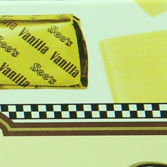
\includegraphics[width=1\textwidth]{images/resize_CC_Noisy_Canon_EOS_5D_Mark3_ISO_3200_C1_47.png}
\end{minipage}
\begin{minipage}{0.055\textwidth}
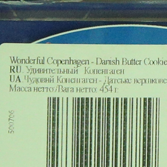
\includegraphics[width=1\textwidth]{images/resize_CC_Noisy_Canon_EOS_5D_Mark3_ISO_3200_C1_52.png}
\end{minipage}
\begin{minipage}{0.055\textwidth}
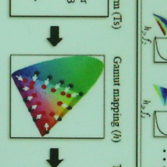
\includegraphics[width=1\textwidth]{images/resize_CC_Noisy_Canon_EOS_5D_Mark3_ISO_3200_C2_44.png}
\end{minipage}
\begin{minipage}{0.055\textwidth}
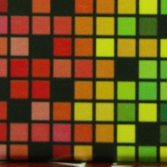
\includegraphics[width=1\textwidth]{images/resize_CC_Noisy_Canon_EOS_5D_Mark3_ISO_3200_C2_66.png}
\end{minipage}
\begin{minipage}{0.055\textwidth}
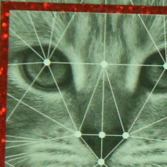
\includegraphics[width=1\textwidth]{images/resize_CC_Noisy_Canon_EOS_5D_Mark3_ISO_3200_C3_26.png}
\end{minipage}
\begin{minipage}{0.055\textwidth}

\includegraphics[width=1\textwidth]{images/resize_CC_Noisy_Canon_EOS_5D_Mark3_ISO_3200_C3_73.png}
\end{minipage}
\begin{minipage}{0.055\textwidth}
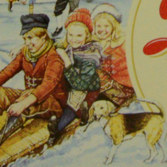
\includegraphics[width=1\textwidth]{images/resize_CC_Noisy_Nikon_D600_ISO_3200_C1_95.png}
\end{minipage}
\begin{minipage}{0.055\textwidth}
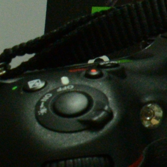
\includegraphics[width=1\textwidth]{images/resize_CC_Noisy_Nikon_D600_ISO_3200_C2_67.png}
\end{minipage}
}\vspace{-3mm}
\subfigure{
\begin{minipage}{0.055\textwidth}
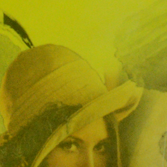
\includegraphics[width=1\textwidth]{images/resize_CC_Noisy_Nikon_D800_ISO_1600_B2_80.png}
\end{minipage}
\begin{minipage}{0.055\textwidth}
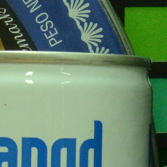
\includegraphics[width=1\textwidth]{images/resize_CC_Noisy_Nikon_D800_ISO_1600_B3_82.png}
\end{minipage}
\begin{minipage}{0.055\textwidth}
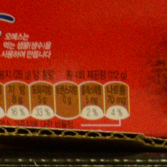
\includegraphics[width=1\textwidth]{images/resize_CC_Noisy_Nikon_D800_ISO_3200_A1_21.png}
\end{minipage}
\begin{minipage}{0.055\textwidth}
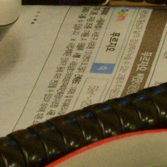
\includegraphics[width=1\textwidth]{images/resize_CC_Noisy_Nikon_D800_ISO_3200_A1_111.png}
\end{minipage}
\begin{minipage}{0.055\textwidth}
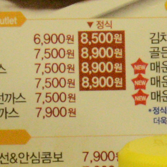
\includegraphics[width=1\textwidth]{images/resize_CC_Noisy_Nikon_D800_ISO_3200_A3_66.png}
\end{minipage}
\begin{minipage}{0.055\textwidth}
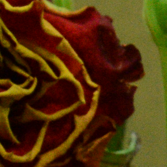
\includegraphics[width=1\textwidth]{images/resize_CC_Noisy_Nikon_D800_ISO_3200_A4_51.png}
\end{minipage}
\begin{minipage}{0.055\textwidth}
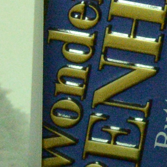
\includegraphics[width=1\textwidth]{images/resize_CC_Noisy_Nikon_D800_ISO_6400_B3_95.png}
\end{minipage}
\begin{minipage}{0.055\textwidth}
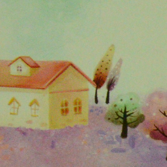
\includegraphics[width=1\textwidth]{images/resize_CC_Noisy_Nikon_D800_ISO_3200_A2_80.png}
\end{minipage}
}
\caption{Some samples cropped from real noisy images of \cite{crosschannel2016}.}
\vspace{-2mm}
\label{fig4}
\end{figure}

\begin{figure*}
\centering
\subfigure{
\begin{minipage}[t]{0.195\textwidth}
\centering
\raisebox{-0.15cm}{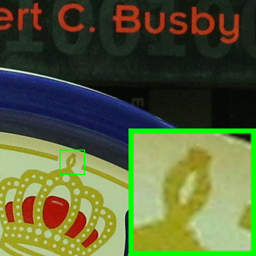
\includegraphics[width=1\textwidth]{images/resize_br_Noisy_5dmark3_iso3200_1_real.png}}
{\footnotesize (a) Noisy  \cite{crosschannel2016}: 37.00dB }
\end{minipage}
\begin{minipage}[t]{0.195\textwidth}
\centering
\raisebox{-0.15cm}{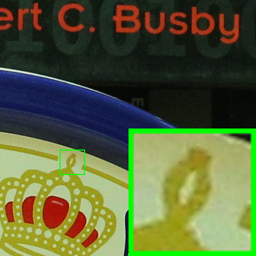
\includegraphics[width=1\textwidth]{images/resize_br_CBM3D_5dmark3_iso3200_1_real.png}}
{\footnotesize (b) BM3D \cite{bm3d,cbm3d}: 37.02dB}
\end{minipage}
\begin{minipage}[t]{0.195\textwidth}
\centering
\raisebox{-0.15cm}{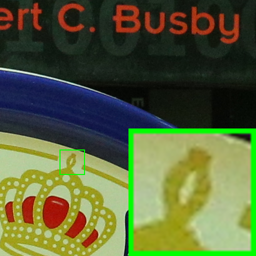
\includegraphics[width=1\textwidth]{images/resize_br_WNNM_5dmark3_iso3200_1_real.png}}
{\footnotesize (c) WNNM \cite{wnnm}: 37.01dB}
\end{minipage}
\begin{minipage}[t]{0.195\textwidth}
\centering
\raisebox{-0.15cm}{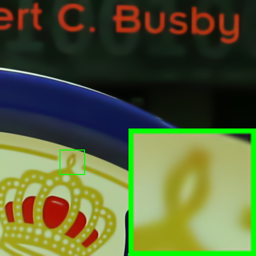
\includegraphics[width=1\textwidth]{images/resize_br_MLP_5dmark3_iso3200_1_real.png}}
{\footnotesize (d) MLP \cite{mlp}: 33.90dB }
\end{minipage}
\centering
\begin{minipage}[t]{0.195\textwidth}
\raisebox{-0.15cm}{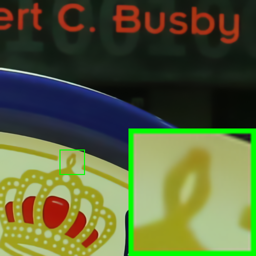
\includegraphics[width=1\textwidth]{images/resize_br_TRD_5dmark3_iso3200_1_real.png}}
{\footnotesize (e) TRD \cite{chen2015learning}: 36.18dB  }
\end{minipage}
}\vspace{-3mm}
\subfigure{
\begin{minipage}[t]{0.195\textwidth}
\centering
\raisebox{-0.15cm}{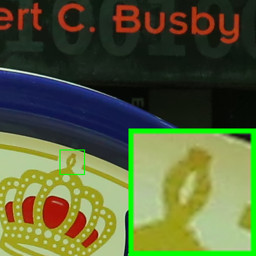
\includegraphics[width=1\textwidth]{images/resize_br_NC_5dmark3_iso3200_1_real.png}}
{\footnotesize (f) NC \cite{noiseclinic}: 38.76dB }
\end{minipage}
\begin{minipage}[t]{0.195\textwidth}
\centering
\raisebox{-0.15cm}{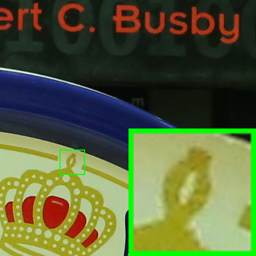
\includegraphics[width=1\textwidth]{images/resize_br_NI_5dmark3_iso3200_1_real.png}}
{\footnotesize (g) NI \cite{neatimage}: 37.68dB  }
\end{minipage}
\begin{minipage}[t]{0.195\textwidth}
\centering
\raisebox{-0.15cm}{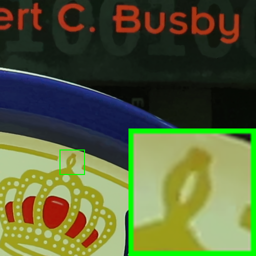
\includegraphics[width=1\textwidth]{images/resize_br_CCNoise_5dmark3_iso3200_1.png}}
{\footnotesize (h) CC \cite{crosschannel2016}: 38.37dB }
\end{minipage}
\begin{minipage}[t]{0.195\textwidth}
\centering
\raisebox{-0.15cm}{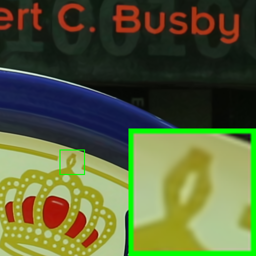
\includegraphics[width=1\textwidth]{images/resize_br_Guided_5dmark3_iso3200_1_real.png}}
{\footnotesize (i) Ours: \textbf{40.50}dB}
\end{minipage}
\begin{minipage}[t]{0.195\textwidth}
\centering
\raisebox{-0.15cm}{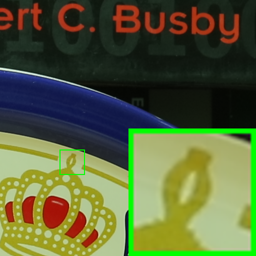
\includegraphics[width=1\textwidth]{images/resize_br_Mean_5dmark3_iso3200_1_real.png}}
{\footnotesize (j) Mean Image \cite{crosschannel2016}}
\end{minipage}
}\vspace{-1mm}
\caption{Denoised images of the image "Canon 5D Mark 3 ISO 3200 1" by different methods. The images are better to be zoomed in on screen.}
%\vspace{-1mm}
\label{fig5}
\end{figure*}

\subsection{Implementation Details}
Our proposed method contains two stages, the external prior learning stage and the external prior guided internal learning stage. In the first stage, we set $p = 6$ (so the patch size is $6\times 6 \times 3$), $M=10$ (the number of patches in a patch group (PG)), $W=31$ (so the window size for PG searching is $31\times31$, and $K=32$ (the number of Gaussians in Gaussian Mixture Model (GMM)). We learn the external prior via GMM on about 3.6 million PGs extracted from the Kodak PhotoCD Dataset (\url{http://r0k.us/graphics/kodak/}), which includes 24 high quality color images. In the second stage, we set $r=54$ (the number of internal atoms in the learned dictionaries), $\lambda=0.001$ (the sparse regularization parameter), $T=2$ (the number of iterations for solving problem (\ref{equ5})), and $IteNum=4$ (the number of iterations for Alg. 1). Our proposed method needs about 60 seconds to denoise an image of size $512\times512\times3$ under the Matlab2014b environment on a machine with Intel(R) Core(TM) i7-5930K CPU of 3.5GHz and 32GB RAM.

\subsection{Comparison with External and Internal Priors}
In this section, we compare our proposed method on real image denoising with external prior based method (denoted as "External") and internal prior based method (denoted as "Internal"). All the three methods perform real image denoising under the weighted sparse coding framework in Equ. (\ref{equ5}). The "External" method employs the external dictionaries (i.e., $r=0$ in Equ. (\ref{equ5})) to recover the latent clean images, while the "Internal" method employ the GMM (with also $K=32$ Gaussians) to directly cluster the internal noisy PGs into multiple subspaces, and perform denoising with internal dictionary learning (i.e., $r=3p^{2}$ in Equ. (\ref{equ5})) for each subspace. All parameters of the three methods are tuned to achieve corresponding best performance.

We compare the above mentioned three methods on the 60 cropped images from \cite{crosschannel2016}. The average PSNR results of these methods are listed in Table \ref{tab1}. It can be seen that our proposed method achieves higher PSNR results then the methods of "External" and "Internal". We also compare the visual quality of the images denoised by these methods. From the results listed in Figure \ref{fig2} and Figure \ref{fig3}, we can see that the "External" method is good at recovering structures (Figure \ref{fig2}) while the "Internal" method is good at recovering internal complex textures (Figure \ref{fig3}). And by making use of both the external and internal priors, our proposed method can recover well both the structures and textures.

In summary, the proposed algorithm achieves better performance on denoising real noisy images than the external prior based method and internal prior based method. 

\begin{table}
\caption{Average PSNR(dB) results of External, Internal, and our proposed methods on 60 real noisy images cropped from \cite{crosschannel2016}.}
\label{tab1}
\vspace{-2mm}
\begin{center}
\renewcommand\arraystretch{1}
\begin{tabular}{|c||c|c|c|c|}
\hline
 & \textbf{Noisy} &\textbf{External} &\textbf{Internal} &\textbf{Ours}  
\\
\hline
PSNR & 34.51 & 38.21 & 38.07 & \textbf{38.75} 
\\
\hline
%SSIM & 0.8718 &  0.9663   & 0.9625 & \textbf{0.9691}
%\\
%\hline
\end{tabular}
\end{center}\vspace{-4mm}
\end{table}



\begin{table*}
\caption{Average PSNR(dB) results of different methods on 60 real noisy images cropped from \cite{crosschannel2016}.}
\label{tab2}
\begin{center}
\renewcommand\arraystretch{1}
\begin{tabular}{|c||c|c|c|c|c|c|c|c|c|c|}
\hline
 & \textbf{Noisy} &\textbf{BM3D}&\textbf{WNNM}&\textbf{MLP}&\textbf{CSF}&\textbf{TRD}& \textbf{NI}& \textbf{NC} &\textbf{Ours} 
\\
\hline
PSNR & 34.51 & 34.58 & 34.52 & 36.19 & 37.40 & {\color{blue}{37.75}} & 36.53 & 37.57  & {\color{red}{ 38.75}}
%\\
%\hline
%SSIM & 0.8718  & 0.8748  & 0.8743   & 0.9470 & 0.9598 &  0.9617 & 0.9241  &  0.9514  & {\color{blue}{0.9685}} & {\color{red}{0.9691}}
\\
\hline
\end{tabular}
\end{center}\vspace{-4mm}
\end{table*}

\subsection{Comparison with Other Denoising Methods}
%For BM3D, we employ its color version \cite{cbm3d} which would have better performance on color images. 

In this section, we compare the proposed method with other state-of-the-art image denoising methods such as BM3D \cite{bm3d}, WNNM \cite{wnnm}, MLP \cite{mlp}, CSF \cite{csf}, TRD \cite{chen2015learning}, Noise Clinic (NC) \cite{noiseclinic}, Cross-Channel (CC) \cite{crosschannel2016}. These methods are designed for removing Gaussian noise. For BM3D and WNNM, the level $\sigma$ of Gaussian noise is very important and is estimated by the method \cite{noiselevel}. The other parameters are set as default. For the methods of MLP, CSF, and TRD, we employ their default parameters settings. Since these methods are designed for grayscale images, we utilize them to denoise the R, G, B channels separately for color noisy images. The Noise Clinic (NC) \cite{noiseclinic} is a blind image denoising method which does not need any noise prior. The recently proposed Cross-Channel (CC) \cite{crosschannel2016} is a state-of-the-art method on real image denoising problem. We also compare with Neat Image (NI), a commercial software for image denoising. Due to its excellent performance, NI is embedded into Photoshop and Corel PaintShop \cite{neatimage}.

The comparisons are performed on the two datasets mentioned before. For the first dataset \cite{crosschannel2016}, the average PSNR results on the 60 cropped images  are listed in Table \ref{tab2} (the code of \cite{crosschannel2016} is not available so that it is not compared). The numbers in red color and blue color are the best and second best results, respectively. It can be seen that our proposed method achieves much better PSNR results than the other methods. The improvement of our method over the second best method (TRD) is 1dB. To compare with \cite{crosschannel2016}, we also perform experiments on the 15 cropped images used in \cite{crosschannel2016}. The PSNR values are listed in Table \ref{tab3}. As we can see, on most (9 out of the 15) images captured by different cameras and camera settings, our proposed method obtains better PSNR values than the other methods. Noted that, though in \cite{crosschannel2016} a specific model is trained for each camera and camera setting, our proposed general method still gains 0.28dB improvements on PNSR over \cite{crosschannel2016}. We also compare the visual quality of the denoised images by the competing methods. Figure \ref{fig5} shows the denoised images of a scene captured by Canon 5D Mark 3 at ISO $=3200$ by the competing methods. More visual comparisons can be found in the supplementary file. We can see that BM3D, WNNM, NC, NI, and CC would either remain noise or generate artifacts, while MLP, TRD are likely to over-smooth the image. Owe to the unify of external and internal priors, our proposed method preserves edges and textures better than other methods. 

For the second dataset \cite{ncwebsite} with no "ground truth" images, we only compare the visual quality of the denoised images. Figure \ref{fig6} shows the denoised images of "Dog" by the competing methods. More visual comparisons can be found in the supplementary file. It can be seen that the methods of BM3D, WNNM tend to globally over-smooth the image while locally remain some noise, while the methods of MLP, TRD are likely to remain noise in the whole image. This demonstrates that the methods designed for Gaussian noise are not effective for removing the complex noise in real noisy images. Though Noise Clinic and Neat Image are specifically developed for removing complex noise, they would sometimes fail to recovery real noisy images. However, our proposed method recoveries more faithfully the structures and textures (such as the eye area) than the other competing methods.

In summary, our proposed method demonstrates impressing ability on dealing with the complex noise in real noisy images in terms of PSNR and visual quality.


\begin{table*}
\caption{Average PSNR(dB) results of different methods on 15 cropped real noisy images used in \cite{crosschannel2016}.}
\label{tab3}
\begin{center}
\renewcommand\arraystretch{1}
\begin{tabular}{|c||c|c|c|c|c|c|c|c|c|c|}
\hline
Camera Settings & \textbf{Noisy} &\textbf{BM3D}&\textbf{WNNM}&\textbf{MLP}&\textbf{CSF}&\textbf{TRD}& \textbf{NI}& \textbf{NC}& \textbf{CC} &\textbf{Ours} 
\\
\hline
\multirow{3}{*}{\small{Canon 5D Mark III}} 
& 37.00 & 37.08 & 37.09 & 33.92 & 35.68 & 36.20 & 37.68 & {\color{blue}{38.76}} & 38.37 & {\color{red}{40.50}}
\\ 
\cdashline{2-11} 
\multirow{3}{*}{ISO = 3200}   
& 33.88 & 33.94 & 33.93 & 33.24 & 34.03 & 34.35 & 34.87 & {\color{blue}{35.69}} & 35.37 & {\color{red}{37.05}}
\\ 
\cdashline{2-11}    
& 33.83 & 33.88 & 33.90 & 32.37 & 32.63 & 33.10 & 34.77 & {\color{blue}{35.54}} & 34.91 & {\color{red}{36.11}}  
\\
\hline
\multirow{3}{*}{Nikon D600} 
& 33.28 & 33.33 & 33.34 & 31.93 & 31.78 & 32.28 & 34.12 & {\color{red}{35.57}} & {\color{blue}{34.98}} & 34.88
\\ 
\cdashline{2-11} 
\multirow{3}{*}{ISO = 3200}   
& 33.77 & 33.85 & 33.79 & 34.15 & 35.16 & 35.34 & 35.36 & {\color{red}{36.70}} & 35.95 & {\color{blue}{36.31}}
\\ 
\cdashline{2-11}    
& 34.93 & 35.02 & 34.95 & 37.89 & 39.98 & {\color{blue}{40.51}} & 38.68 & 39.28 & {\color{red}{41.15}} & 39.23
\\
\hline
\multirow{3}{*}{Nikon D800} 
& 35.47 & 35.54 & 35.57 & 33.77 & 34.84 & 35.09 & 37.34 & {\color{blue}{38.01}} & 37.99 & {\color{red}{38.40}}
\\ 
\cdashline{2-11} 
\multirow{3}{*}{ISO = 1600}   
& 35.71 & 35.79 & 35.77 & 35.89 & 38.42 & 38.65 & 38.57 & 39.05 & {\color{blue}{40.36}} & {\color{red}{40.92}}
\\ 
\cdashline{2-11}    
& 34.81 & 34.92 & 34.95 & 34.25 & 35.79 & 35.85 & 37.87 & 38.20 & {\color{blue}{38.30}} & {\color{red}{38.97}}
\\
\hline
\multirow{3}{*}{Nikon D800} 
& 33.26 & 33.34 & 33.31 & 37.42 & 38.36 & 38.56 & 36.95 & 38.07 & {\color{red}{39.01}} & {\color{blue}{38.66}}
\\ 
\cdashline{2-11} 
\multirow{3}{*}{ISO = 3200}   
& 32.89 & 32.95 & 32.96 & 34.88 & 35.53 & 35.76 & 35.09 & 35.72 & {\color{blue}{36.75}} & {\color{red}{37.07}}
\\ 
\cdashline{2-11}    
& 32.91 & 32.98 & 32.96 & 38.54 & {\color{blue}{40.05}} & {\color{red}{40.59}} & 36.91 & 36.76 & 39.06 & 38.52
\\ 
\hline
\multirow{3}{*}{Nikon D800} 
& 29.63 & 29.66 & 29.71 & 33.59 & 34.08 & {\color{blue}{34.25}} & 31.28 & 33.49 & {\color{red}{34.61}} & 33.76
\\ 
\cdashline{2-11} 
\multirow{3}{*}{ISO = 6400}   
& 29.97 & 30.01 & 29.98 & 31.55 & 32.13 & 32.38 & 31.38 & 32.79 & {\color{blue}{33.21}} & {\color{red}{33.43}}
\\ 
\cdashline{2-11}    
& 29.87 & 29.90 & 29.95 & 31.42 & 31.52 & 31.76 & 31.40 & 32.86 & {\color{blue}{33.22}} & {\color{red}{33.58}}
\\
\hline
Average & 33.41 & 33.48 & 33.48 & 34.32 & 35.33 & 35.65 & 35.49 & 36.43 & {\color{blue}{36.88}} & {\color{red}{ 37.16}}
\\
\hline
%Average SSIM & 0.8483 & 0.8511 & 0.8512 & 0.9113 & 0.9250 & 0.9280 & 0.9126 & 0.9364 & {\color{blue}{0.9481}} & {\color{red}{ 0.9505}}
%\\
%\hline
\end{tabular}
\end{center}\vspace{-3mm}
\end{table*}

\begin{figure*}
\centering
\subfigure{
\begin{minipage}[t]{0.244\textwidth}
\centering
\raisebox{-0.15cm}{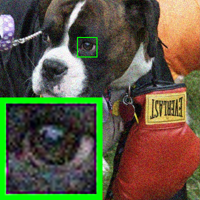
\includegraphics[width=1\textwidth]{images/resize_br_Noisy_dog.png}}
{\footnotesize (a) Noisy \cite{ncwebsite}   }
\end{minipage}
\begin{minipage}[t]{0.244\textwidth}
\centering
\raisebox{-0.15cm}{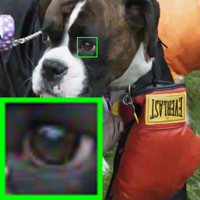
\includegraphics[width=1\textwidth]{images/resize_br_BM3D_dog.png}}
{\footnotesize (b) BM3D \cite{bm3d,cbm3d}  }
\end{minipage}
\begin{minipage}[t]{0.244\textwidth}
\centering
\raisebox{-0.15cm}{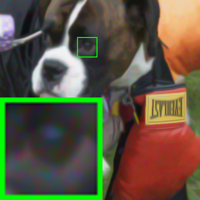
\includegraphics[width=1\textwidth]{images/resize_br_WNNM_dog.png}}
{\footnotesize (c) WNNM \cite{wnnm}   }
\end{minipage}
\begin{minipage}[t]{0.244\textwidth}
\centering
\raisebox{-0.15cm}{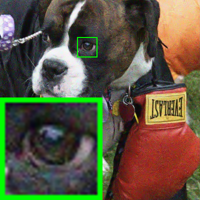
\includegraphics[width=1\textwidth]{images/resize_br_MLP_dog.png}}
{\footnotesize (d) MLP \cite{mlp}  }
\end{minipage}
}\vspace{-3mm}
\subfigure{
\begin{minipage}[t]{0.244\textwidth}
\centering
\raisebox{-0.15cm}{\includegraphics[width=1\textwidth]{images/resize_br_TRD_dog.png}}
{\footnotesize (e) TRD \cite{chen2015learning}}
\end{minipage}
\begin{minipage}[t]{0.244\textwidth}
\centering
\raisebox{-0.15cm}{\includegraphics[width=1\textwidth]{images/resize_br_NC_dog.png}}
{\footnotesize (f) NC \cite{noiseclinic}  }
\end{minipage}
\begin{minipage}[t]{0.244\textwidth}
\centering
\raisebox{-0.15cm}{\includegraphics[width=1\textwidth]{images/resize_br_NI_dog.png}}
{\footnotesize (g) NI \cite{neatimage}   }
\end{minipage}
\begin{minipage}[t]{0.244\textwidth}
\centering
\raisebox{-0.15cm}{\includegraphics[width=1\textwidth]{images/resize_br_Guided_dog.png}}
{\footnotesize (h) Ours  }
\end{minipage}
}
\caption{Denoised images of the image "Dog" by different methods. The images are better to be zoomed in on screen.}
\vspace{-2mm}
\label{fig6}
\end{figure*}

\section{Conclusion and Future Work}

The image priors are commonly used for image denoising problem. The external priors are general but not adaptive to specific images, while the internal priors are adaptive but would largely degraded by the complex noise in real noisy images. In this paper, we demonstrates that, we can unify the priors in external clean images and in internal noisy images to achieve better performance on real image denoising problem. This unify can be attempted by employing the external prior learned on natural images to guide the internal prior learning on given noisy images. The experiments on standard datasets have demonstrated the powerful ability of the proposed method. In the future, we will evaluate the proposed method on other computer vision tasks such as image super-resolution, image deblurring, etc.

\clearpage
{
\small
\bibliographystyle{unsrt}
\bibliography{egbib}
}

\end{document}
